\documentclass[a4paper, 11pt, ngerman, parskip=half-]{scrartcl}

\title{MoF - Fragenkatalog}
\subtitle{\href{https://github.com/Bierbunker/MoF-Ausarbeitung}{\underline{Aktuelle Version (Link)}}}
\date{\today}

\usepackage[margin=1in]{geometry}

\usepackage[utf8]{inputenc}
\usepackage[T1]{fontenc}
\usepackage{lmodern}
\usepackage{babel}
\usepackage{csquotes}
\usepackage{xurl}

\usepackage{amsmath, amssymb, amstext, mathtools}
\usepackage{icomma}
\usepackage[locale=DE]{siunitx}
\usepackage{physics}
\usepackage{derivative}  % overrides derivatives of package physics!

\usepackage{pdfpages}
\usepackage{lastpage}
\usepackage{graphicx}
\usepackage{float}
\usepackage{mhchem}
\usepackage{xcolor}
\usepackage[hidelinks,colorlinks]{hyperref}
%Colorlinks setup:
\hypersetup{
    colorlinks = false,
    linkbordercolor = {white}
}

\usepackage[headsepline]{scrlayer-scrpage}
\pagestyle{scrheadings}
\setkomafont{pageheadfoot}{\normalfont}
\ihead{\hyperlink{Fehler}{\color{cyan}Fehlermeldungen}}
\chead{MoF Fragenkatalog}
\ohead{\today}
\cfoot{\pagemark{} / \pageref*{LastPage}}

\usepackage{caption, subcaption}
\captionsetup[table]{name=Tabelle}
\captionsetup[figure]{name=Abbildung}
\captionsetup{format=plain, font=small, labelfont=bf, justification=centering}

% Line break after paragraph
\newcommand{\myparagraph}[1]{\paragraph{#1}\mbox{}\\}

% numerical aperture
\newcommand{\NA}{\ensuremath{\mathit{NA}}}


% Question command
\newcounter{question}
\newcommand{\question}[1]{\stepcounter{question}\paragraph{Frage \thequestion: #1}~}

\newcommand{\qref}[1]{%
  \phantomsection\label{q:#1}% Create a label for the question
  \textbf{\hyperref[q:#1]{#1}}% Link to the question label
}

\newcommand{\aqref}[1]{%
  \phantomsection\label{q:#1}% Create a label for the question
  \textbf{\hyperref[q:#1]{Frage #1}}% Link to the question label
}

\begin{document}

\maketitle

\newpage

\tableofcontents
\newpage
\section{Notizen aus der Vorlesung}
Magnetismus wird wahrscheinlich nicht zur Prüfung am 26. kommen. (Cat 15.06.)
\newpage
\section*{Ähnliche Fragen vermutlich (GPT-4)}

Einige Fragen sind ähnlich oder decken ähnliche Themen ab. Hier sind die entsprechenden Paare:

Fragen \qref{1} und \qref{13} diskutieren die Austauschenergie beim H2 Molekül und ihre Bedeutung für die chemische Bindung.

Fragen \qref{2} und \qref{14}, \qref{21}, \qref{32}, \qref{40} und \qref{55} fragen nach Informationen, die aus dem Rotations-Schwingungsspektrum von Molekülen abgeleitet werden können.

Fragen \qref{3} und \qref{15} behandeln elektrische Rotations-Schwingungsübergänge und die Entstehung von Schwingungsbanden.

Fragen \qref{4} und \qref{16}, \qref{27} und \qref{45}, \qref{50} und \qref{54} beziehen sich auf den Zusammenhang zwischen der Gitterebene und einem Vektor im reziproken Raum.

Fragen \qref{5} und \qref{17}, \qref{47} und \qref{59} beziehen sich auf das Auftreten von Energiebandlücken mit Hilfe des Models der fast freien Elektronen.

Fragen \qref{6} und \qref{18} behandeln, wie experimentell die Dispersionsrelationskurve von Phononen ermittelt werden kann.

Fragen \qref{7} und \qref{19}, \qref{38}, \qref{51} und \qref{57} diskutieren die Wärmekapazität sowohl in der klassischen als auch in der quantenmechanischen Betrachtung.

Fragen \qref{8} und \qref{20} beziehen sich auf das Bloch-Theorem eines Elektrons im harmonischen Potential.

Fragen \qref{9} und \qref{56} behandeln den Paulschen Paramagnetismus.

Fragen \qref{24} und \qref{37} beziehen sich auf die Hybridisierung in mehratomigen Molekülen.

Fragen \qref{25} und \qref{35}, \qref{44} behandeln die Laue'sche Beugungsbedingung und die Ewald-Konstruktion.

Fragen \qref{26} und \qref{36} diskutieren den Unterschied zwischen einem fcc-Gitter und einer hcp-Struktur.

Fragen \qref{28} und \qref{39}, \qref{48} und \qref{58} vergleichen die Einstein- und Debye-Modelle der spezifischen Wärme.

Fragen \qref{30} und \qref{49} erläutern den Atomfaktor und den Strukturfaktor bei der Röntgenbeugung.

Fragen \qref{41} und \qref{52} behandeln die Lennard-Jones-Potential und Van der Waals Bindung.

Fragen \qref{42} und \qref{33} behandeln das Konzept des Bravaisgitters und der Wigner-Seitz Zelle.

Fragen \qref{43} und \qref{31}, \qref{34} diskutieren das Franck-Condon Prinzip und die Intensität von Schwingungsbänden in einem Molekülspektrum.

Es ist wichtig zu beachten, dass obwohl diese Fragen ähnliche Themen behandeln, die spezifischen Aspekte oder der Kontext, der in jeder Frage behandelt wird, variieren können. Daher ist es wichtig, jede Frage sorgfältig zu lesen und zu verstehen, bevor man versucht, sie zu beantworten.

\newpage
\section{01. Mai 2015}
\question{Austauschenergie beim H2 Molekül? Wann ist es groß/klein? Wieso ist es für die Bindung wichtig?}
\label{q:1}

Die Austauschenergie oder oft auch \textbf{Austauschwechselwirkung} spielt bei der chemischen Bindung eine bedeutende Rolle. \\
Sie ist groß, falls sich die Atomorbitale stark überlappen---sprich symmetrisch sind---und kleiner falls sie sich weniger überlappen (=anti-symmetrisch). \\
Wie man in der Abbildung erkennen kann, ergibt sich eine Bindung nur, wenn die Orbitale sich überlappen (im symmetrischen Fall $U_S$). \\
\begin{figure}[H]  
    \centering
    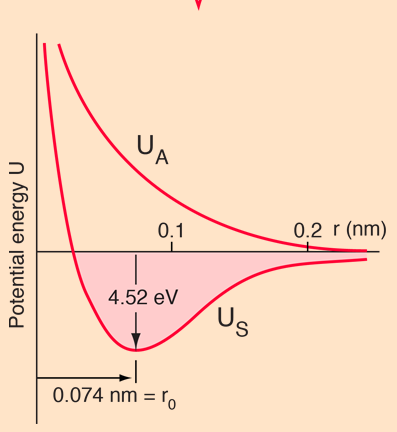
\includegraphics[width=.4\textwidth]{resources/05-01-2015/Frage1.png}
    \caption{siehe \href{http://hyperphysics.phy-astr.gsu.edu/hbase/molecule/hmol.html}{LINK}}
\end{figure}

\question{Was kann man aus dem Rotations-Schwingungsspektrum für molekulare Größen bestimmen?}
\label{q:2}

Unter Annahme, dass die beiden Atome ihren Abstand bei Rotation nicht ändern kann man den \textbf{Bindungsabstand} $R_e$ bestimmen. \\
Weiter lässt sich die \textbf{Rotationskonstante} $B_e$ bzw. deren anharmonischer Anteil $\alpha_e$, die \textbf{Schwingungsfrequenz} $\omega$ und das \textbf{Trägheitsmoment} $I$ bestimmen. \\

\[B_e = \frac{\hbar}{4 \pi c M R_e^2}\text{\quad [cm$^{-1}$]}\]
\[E_{rot} = \frac{\hbar^2}{2 I} \cdot J(J+1)\text{\quad [J]}\]
\[E_{rot} = B_e \cdot h\cdot c\]
$J$ ist dabei die Quantenzahl der Rotation und $M$ die reduzierte Masse (damit $M * R_e^2$ eben $I$ entspricht; gilt freilich nur für 2-Atom Systeme). \\

\[\Delta E_{rot} = \frac{(J+1)\hbar^2}{M\cdot {R_e}^2}\]
\[\Delta E_{vib} = \hbar \cdot \omega\]

\question{Diskutieren Sie elektrische Rotations-Schwingungsübergänge und die Entstehung von Schwingungsbanden.}
\label{q:3}

Übergänge zwischen Schwingungs-Rotations-Niveaus ($f_i$,$J_i$) $\rightarrow$ ($f_j$,$J_j$) innerhaltb desselben elektronischen Zustandes bilden für $f_i \neq f_j$ ein Schwingungs-Rotations-Spektrum. \\

\textbf{WICHTIG:} nur Moleküle welche ein permanentes Dipolmoment besitzen können solche Übergänge durchführen (z.B.: \ce{CO2}, \ce{H2O} aber \underline{nicht} \ce{O2}, andere homonuklearen, \dots etc.). \\

Wird Energie (Photon) von außen zugeführt oder abgegeben, so kann ein Übergang zwischen den Niveaus stattfinden - Auswahlregel $\Delta J = \pm 1$. Sprich Rotations-Schwingungsübergänge spielen sich zwischen benachbarten Niveaus ab.\\

\textbf{Schwingungsbanden} bezeichnen nun alle Rotationslinien welche zu einem Schwingungsübergang gehören. \\


\question{Was für ein Zusammenhang besteht zwischen der Gitterebene und einem Vektor im reziproken Raum?}
\label{q:4}

Der Abstand zweier Gitterebenen $d_{hkl}$ ist gegeben durch:
\[d_{hkl} = \frac{a}{\sqrt{h^2 + k^2 + l^2}}\]
und hängt mit dem reziproken Gittervektor $\vec{G_{hkl}}$ 
\[\vec{G_{hkl}} = h\vec{b_1} + k\vec{b_2} + l\vec{b_3}\]
wie folgt zusammen:
\[d_{hkl} = \frac{2\pi}{|\vec{G_{hkl}}|}\]

Somit ist die Länge des reziproken Gittervektors $\vec{G_{hkl}}$ indirekt proportional zum Abstand der Gitterebenen $d_{hkl}$.

\question{Erklären Sie das Auftreten von Energiebandlücken mit Hilfe des Models der fast freien Elektronen.}
\label{q:5}

\question{Wie kann experimentell die Dispersionsrelationskurve von Phononen ermittelt werden?}
\label{q:6}

\begin{figure}[H]  
    \centering
    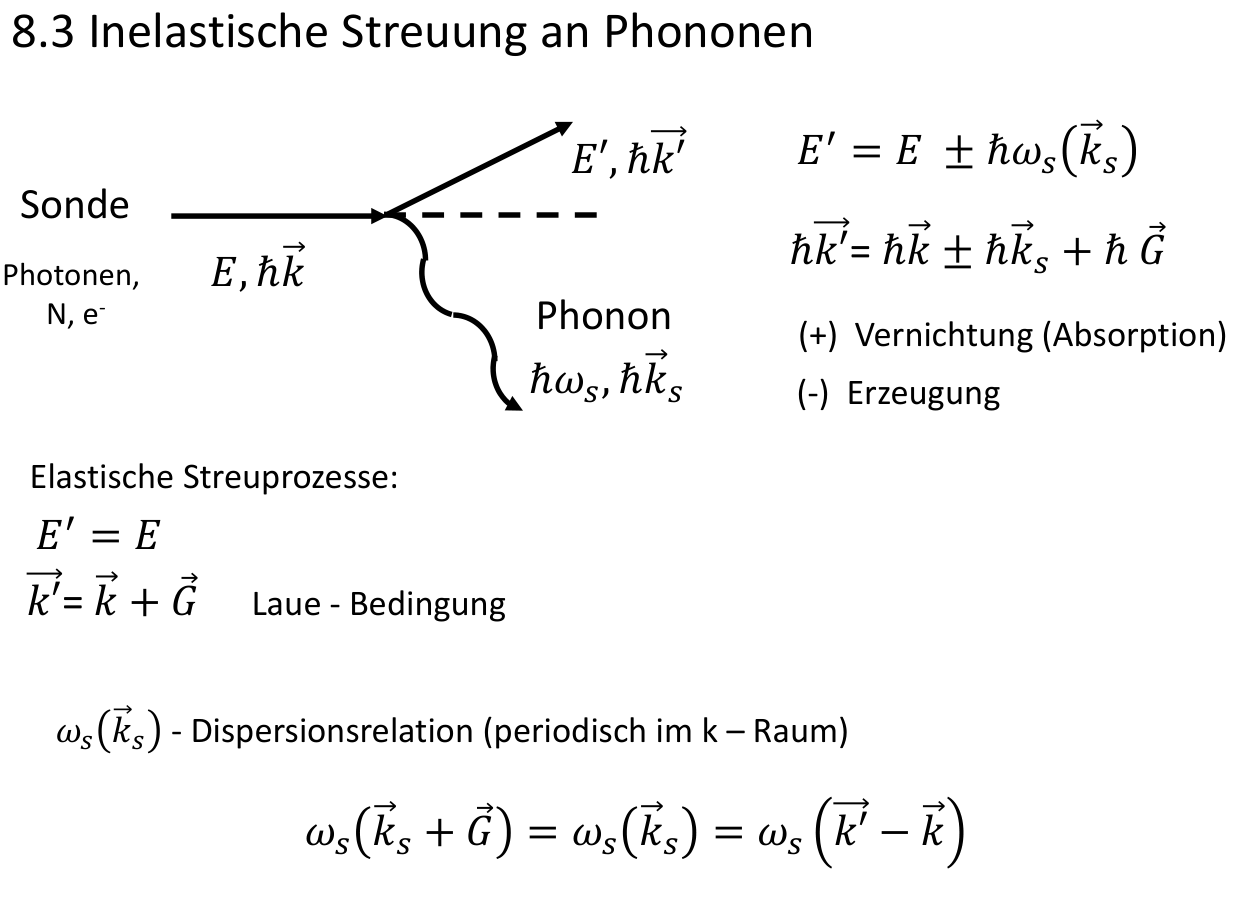
\includegraphics[width=.8\textwidth]{resources/05-01-2015/Frage6_1.png}
    \caption{Inelastische Streuung an Phononen}
\end{figure}

\begin{figure}[H]  
    \centering
    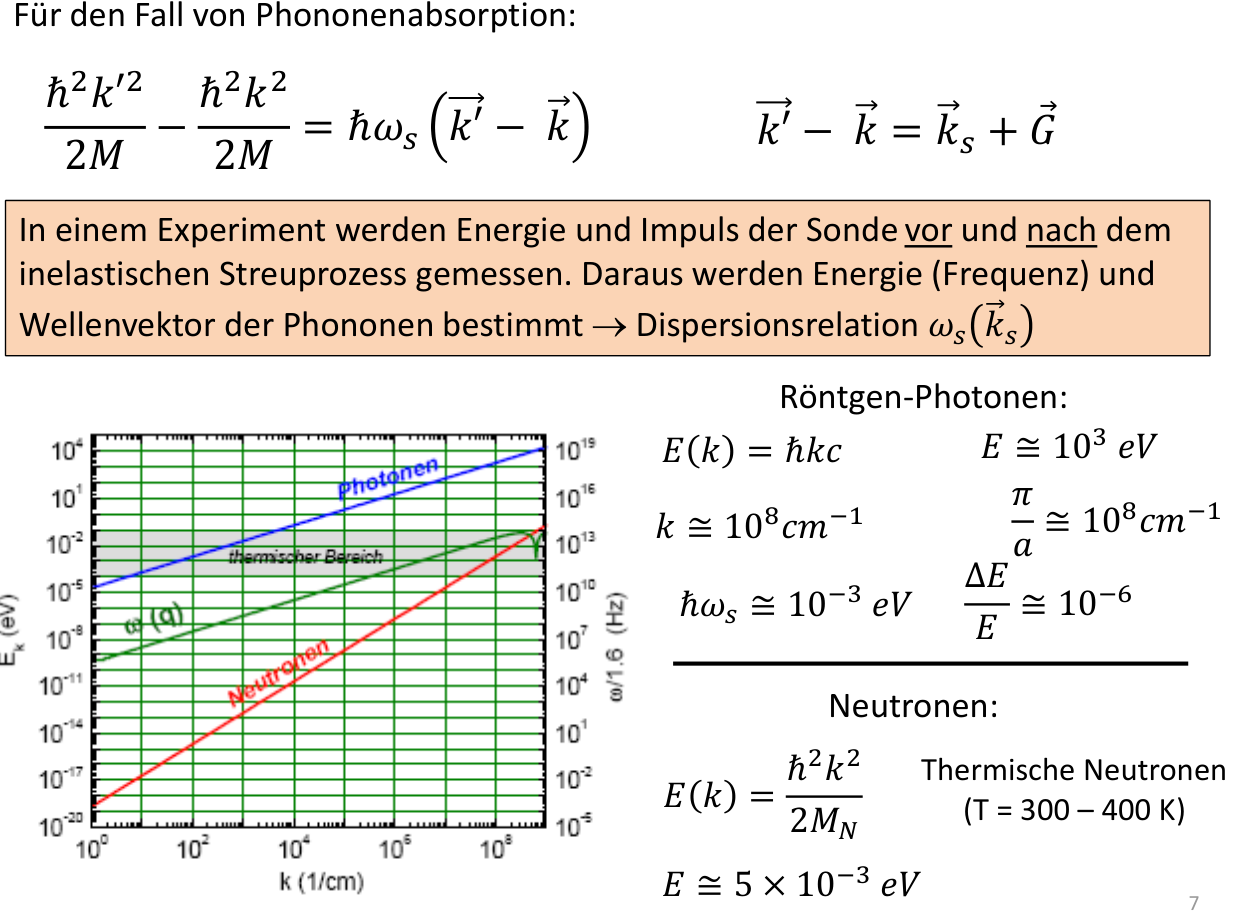
\includegraphics[width=.8\textwidth]{resources/05-01-2015/Frage6_2.png}
    \caption{Dispersionsrelation Phononen in einem Experiment}
\end{figure}

\question{Diskutieren Sie die Wärmekapazität sowohl in der klassischen als auch in der quantenmechanischen Betrachtung.}
\label{q:7}

In der der klassischen Physik wird angenommen, dass die Energieauf- und abnahme eines Materials 
kontinuerlich ist bzw. die Energieniveaus von Molekülen und Atomen eines Materials kontinuierlich 
variieren können. \\
In den quantenmechanischen Modellen können die Energieniveaus nur diskrete Werte annehmen, wodurch die 
Wärmekapazität eines Materials bei niedrigen Temperaturen diskrete Schritte 
aufweist, die durch die Energieniveaus der quantenmechanischen Zustände bestimmt sind (Einstein, Debye).
(Die Quantisierung der Gitterschwingungen ist entscheidend für die innere Energie und
die spezifische Wärme des Kristallgitters.)
\\
Bei hohen Temperaturen nähert sich die klassische Wärmekapazität der quantenmechanischen Wärmekapazität 
an (Abstände zwischen Energieniveaus wird kleiner).

\begin{figure}[H]  
    \centering
    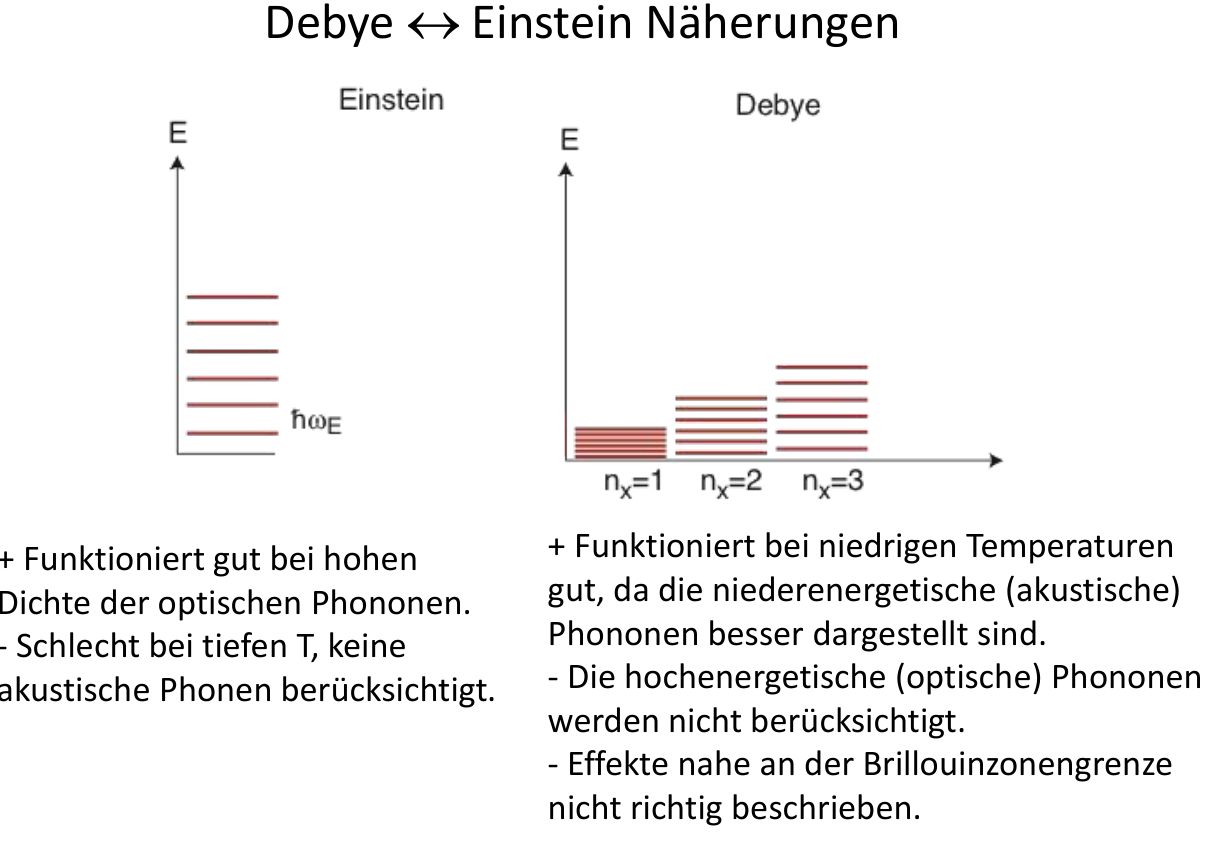
\includegraphics[width=.8\textwidth]{resources/05-01-2015/Frage7.png}
    \caption{Vergleich zwischen Einstein- und Debye-Modell.}
\end{figure}

\question{Beschreiben Sie das Bloch-Theorem eines Elektrons im harmonischen Potential.}
\label{q:8}

\question{Beschreiben Sie den Paulschen Paramagnetismus.}
\label{q:9}

\question{Potentiat-Bindung im homöopolaren Molekül?}
\label{q:10}
Siehe Frage \ref{q:11}


\newpage
\section{05. Mai 2015}

\question{Skizzieren Sie den Verlauf der Potentialkurve für ein homöopolares Molekül. Erklären Sie sie qualitativ.}
\label{q:11}

Homöopolare Moleküle sind Moleküle, die aus Atomen desselben Elements bestehen. Sie entstehen durch kovalente Bindungen. In Abbildung \ref{fig:Frage_11} ist die Potentialkurve einer kovalten Bindung dargestellt welche mit einem Lennard-Jones-Potential angenähert werden kann. Für kleine Abstände dominiert der Faktor $\frac{a}{R^12}$ (Abstoßung der Elektronen durch Pauli Prinzip) bei größeren Abständen der Faktor $-\frac{b}{R^6}$ (Van der Waals). Die Bindungsernergie $E_B$ befindet sich beim globalen Minimum. 
\begin{figure}[h!]
    \centering
    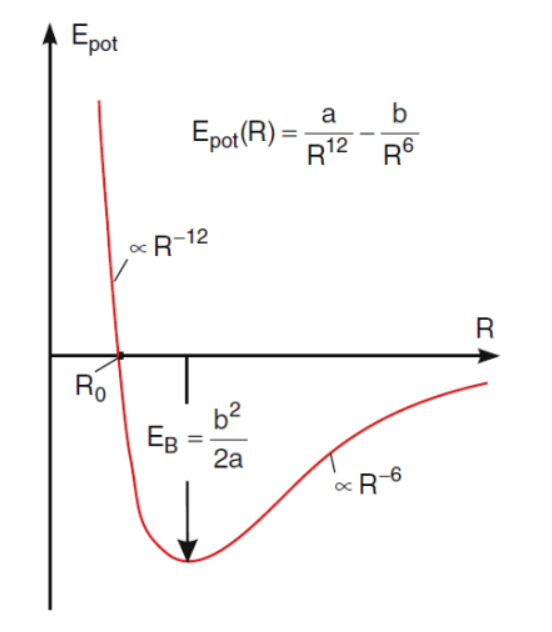
\includegraphics[width = 0.4\textwidth]{resources/05-05-2015/Frage_11.png}
    \caption{Potentialkurve homöopolare Molekül}
    \label{fig:Frage_11}
\end{figure}


\question{Erklären Sie die Herkunft der 'Austauschenergie' in H2. Wann ist sie groß, wann klein? Warum ist sie entscheidend für die chemische Bindung?}
\label{q:12}

Siehe \aqref{1}

\question{Welche Informationen über molekulare Kenngrößen können aus Rotations-Schwingungsspektren von Molekülen erhalten werden?}
\label{q:13}

Es können folgende Kenngrößen bestimmt werden:
\begin{itemize}
\item Gleichgewichtsabstand $R_e$
\item Rotationskonstanten $B_e$ und $\alpha_e$
\item Form der Potentialkurve
\end{itemize}

\question{Diskutiere einen elektronischen Übergang in einem 2-Atomigen Molekül und die daraus resultierenden Schwingungsbanden im Spektrum.}
\label{q:14}

Ändert sich die Schwingungsquantenzahl $\nu$ so ändert sich die Energie $E_{vib}$, bei Änderung der Rotationsquantenzahl $J$ die Energie $E_rot$ Die Gesamternergie setzt sich aus der Schwingungs- Rotations- und Potentiellenenergie zusammen:
\begin{equation}
    E = E_{rot} + E_{vib} + E_{pot}
\end{equation}
Der Abstand zwischen den einzelen Energien $E_{rot}$ ist dabei deutlich kleiner als der zwischen den einzelnen Energien $E_{vib}$.\\
Übergänge zwischen Schwingungs-Ratationsnevaus $(\nu_i, J_i) \longleftrightarrow (\nu_k, J_k), \nu_i \neq \nu_k$: Schwingungsrotationsspektrum im infraroten Spektralbereich (2-10 \textmu m)\\
Übergänge zwischen Schwingungs-Ratationsnevaus $(\nu_i, J_i) \longleftrightarrow (\nu_k, J_k), \nu_i = \nu_k$: Reines Rotationsspektrum, Mikrowellenbereich ($10^3-10^4$ \textmu m)
\begin{figure}[h!]
    \centering
    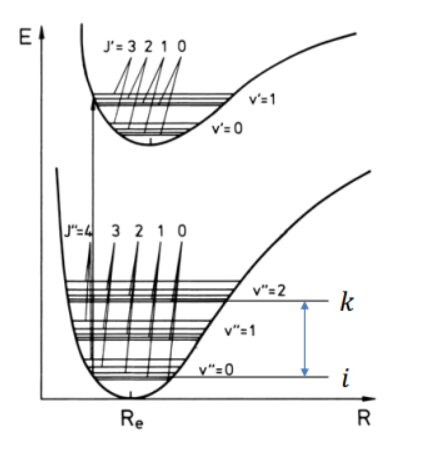
\includegraphics{resources/05-05-2015/Frage_14.png}
    \caption{Übergänge zwischen Schwingungs-RotationsNiveaus}
    \label{fig:enter-label}
\end{figure}

\question{Diskutiere den Zusammenhang zwischen Gitterebene im Kristall und Vektoren des reziproken Gitters.}
\label{q:15}

Siehe \aqref{4}.

\question{Diskutieren Sie die Wärmekapazität des Gitters im Rahmen des klassischen und der Quantenmechanik.}
\label{q:16}

\textbf{Klassische Mechanik}:\\
\begin{itemize}
    \item Keine Translations- und Rotationsfreiheitsgrade
    \item Jedes Atom kann in 3 voneinander unabhängigen Raumrichtungen schwingen:
    \begin{itemize}
        \item 3 Schwingungsfreiheitsgrade der kinetischen Energie
        \item 3 Schwingungsfreiheitsgrade der potentiellen Energie
    \end{itemize}
\end{itemize}
Gesetzt von Dulong-Petit:
\begin{equation}
    f = 6 \qquad c_\nu ^m = 3N_Ak_B = 3R = \SI{24.9}{\frac{J}{K mol}}
\end{equation}

\textbf{Quantenmechanik}
Quantisierung der Gitterschwingungen entscheidend für die innere Energie und
die spezifische Wärme des Kristallgitters.\\
Bei niedrigen Temperaturen ($k_BT<<\hbar\omega$) kommt es zu einem Ausfrieren der Schwingungsfreiheitsgrade:
\begin{equation}
    c_\nu^m \rightarrow 0
\end{equation}
Bei hohen Temperaturen ($k_BT>>\hbar\omega$):
\begin{equation}
    c_\nu^m \rightarrow 3R \qquad \text{gleich wie beim Gesetzt von Dulong-Petit}
\end{equation}


\question{Wie ermittelt man experimentell eine Phononendispersionskurve?}
\label{q:17}
Durch Streuung von Photonen, Neutronen oder Elektronen am Kristallgitter. 

\begin{figure}[h!]
    \centering
    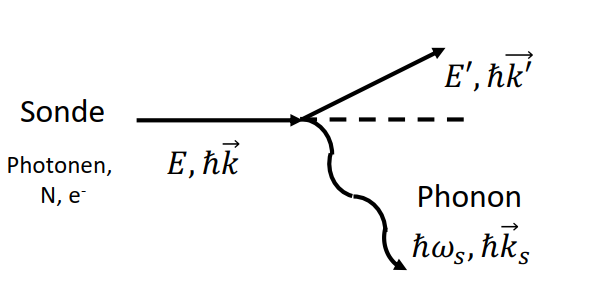
\includegraphics{resources/05-05-2015/Frage_17.png}
    \caption{Inelastische  Streuung an Phononen}
    \label{fig:enter-label}
\end{figure}
Die Dispersionsrelation ergibt sich dann zu:
\begin{equation}
    \omega_s(\Vec{k_s})=\omega_s(\Vec{k'}-\Vec{k})
\end{equation}
Am besten durch Streuung von Neutronen: 
\begin{itemize}
    \item Energie und Impuls von Neutronen im selben Bereich wie Phononen
    \item Neutronen werden nur an Atomkernen gestreut und regen Gitterschwingungen an
\end{itemize}


\question{Erklären Sie das Zustandekommen von Energiebändern in Festkörper im Rahmen der Theorie der fast-freien Elektronen.}
\label{q:18}

\question{Erklären Sie das Bloch'sche Theorem für Elektronen im periodischen Potential.}
\label{q:19}

\question{Diskutieren Sie den Paulschen Paramagnetismus.}
\label{q:20}
\newpage
\section{09. Mai 2012}

\question{Skizzieren der wesentlichen Elemente der Born-Oppenheimer Näherung.}
\label{q:21}

Da die Atomkerne eine wesentlich größere Masse als die Elektronen haben und sich dadurch viel langsamer bewegen, ist es mit der Born-Oppenheimer
Näherung möglich die Positionen der Kerne zu fixieren. Somit lässt sich die molekulare Schrödingergleichung in eine für die Kerne und eine
für die Elektronen aufteilen.

\begin{itemize}
    \item Für die Elektronen stehen die Kerne still, wodurch ihre Lage als Parameter in das anziehende und abstoßende Potential eingeht.
        Somit hängen die elektronischen Eigenzustände und Energien nur von der Lage der Kerne ab und nicht von der Geschwindigkeit.\\
            Die Schrödingergleichung für die Elektronen lautet somit:
            
        \begin{align}
            \hat{H}_e * \Phi_h(\vec{r},\vec{R}) = E_h(\vec{R}) *  \Phi_h(\vec{r},\vec{R})
        \end{align}

        Dabei ist $\vec{r}$ die Position der Elektronen und $\vec{R}$ die der Kerne. Der Hamiton besteht aus $\hat{H}_e = \hat{T}_e + \hat{V}_{ee} + \hat{V}_{eN}$, 
        also der kinetischen Energie der Elektronen + der Abstoßung zwischen den Elektronen + der Anziehung zwischen Kernen und Elektronen.

        \begin{figure}[H]
            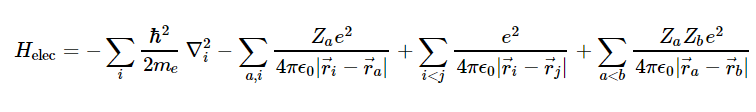
\includegraphics[width=0.8\linewidth]{resources/09-05-2012/born_op.PNG}
            \caption{Elektronischer Hamiton}
        \end{figure}

    \item Die Kernbewegeung ist von den Elektronen nahezu unbeeinflusst, jedoch bewegen sie sich im Potential der elektrischen Zustände. 
        Die Kern-Wellenfunktion $\eta_{hk}(\vec{R})$ hängt nur von der Kernkoordinate $\vec{R}$ ab.\\
        Die Schrödingergleichung lautet: 

        \begin{align}
            (\hat{T}_n + \hat{V}_{NN} + E_h(\vec{R})) * \eta_{hk}(\vec{R}) = E_{hk} * \eta_{hk}(\vec{R})
        \end{align}
\end{itemize}



\question{Welche Informationen über molekulare Kerngrößen können aus Rotations-Schwingungsspektren von Molekülen erhalten werden?}
\label{q:22}

\question{Diskutieren das Schwigungs-Rotations Spektrum eines 2-atomigen Moleküls.}
\label{q:23}

\question{Welche Verbesserungen des einfachen MO- oder VB-Ansatzes ermöglichen eine bessere Übereinstimmung mit den experimentellen Werten?}
\label{q:24}

\question{Was versteht man unter dem Franck-Condon Prinzip? Diskutiere die Intensität von Schwingungsbänden in einem Molekülspektrum bei einem elektronischen Übergang an Hand des Franck-Condon Prinzips.}
\label{q:25}

\question{Diskutiere die Laue'sche Beugungsbedingung: anhand Ewald Konstruktion im Rahmen der Bragg'schen Interpretation.}
\label{q:26}

\question{Erläutere den Atomfaktor und den Strukturfaktor bei der Röntgenbeugung.}
\label{q:27}

\question{Skizziere die 1. Brillouin Zone eines ebenen ParaRechteckgitters.}
\label{q:28}

\question{Wodurch unterscheiden sich akustische von optischen Phononen?}
\label{q:29}

Ein Phonon ist die elementare Anregung (Quant) des elastischen Feldes. Sie beschreiben die elementare bzw. kollektive Anregungen der Gitterschwingungen eines Festkörpers.
In einem dreidimensionalen Kristall mit $N$ Atomen in der primitiven Basis existieren zu jedem mit der Kristallsymmetrie verträglichen Wellenvektor 
$3N$ mögliche Schwingungsmoden:

\begin{itemize}
    \item Akustische Phononen: Diese Phononen werden auch als Schallquanten bezeichnet und sind die Quanten der Schallwellen, die sich durch das Kristallgitter fortpflanzen.
          Alle Quanten bewegen sich hier in einer Einheitszelle in Phase und haben 3 akustische Moden, wovon eine longitudinal und zwei transversal sind.

          \begin{figure}[H]
            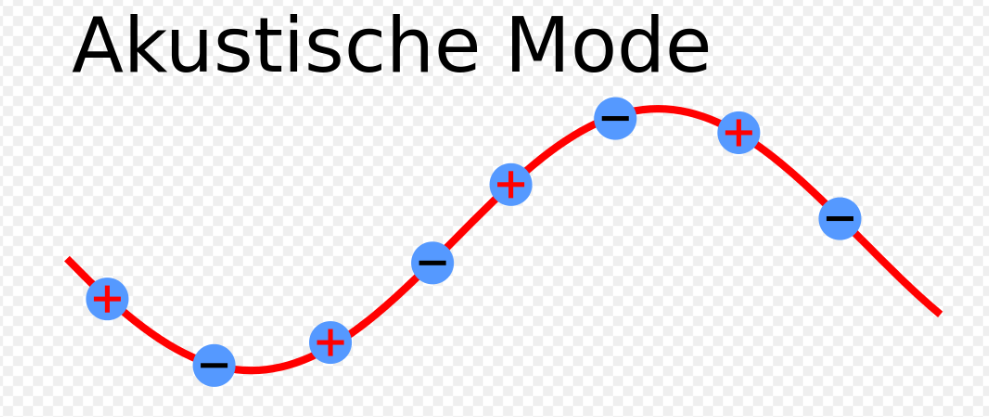
\includegraphics[width=0.8\linewidth]{resources/09-05-2012/akust.PNG}
            \caption{Darstellung von akustischen Transversalwellen von Phononen}
          \end{figure}
    \item Optische Phononen: Diese Phononen bewegen sich in einer Basisgegenphasig, wodurch es Schwingungsmodi gibt, bei denen entgegengesetzt geladene Untergitter gegeneinander schwingen. 
          Die dabei oszillierenden Dipolmomente können mit Photonen wechselwirken. Oft kommen solche Kopplungen im Infrarotbereich, also der Wärmebewegung in Festkörpern vor.
          Beispiele für solche infrarot-aktiven Gitter sind Ionengitter wie Natriumchloridkristalle.

          \begin{figure}[H]
            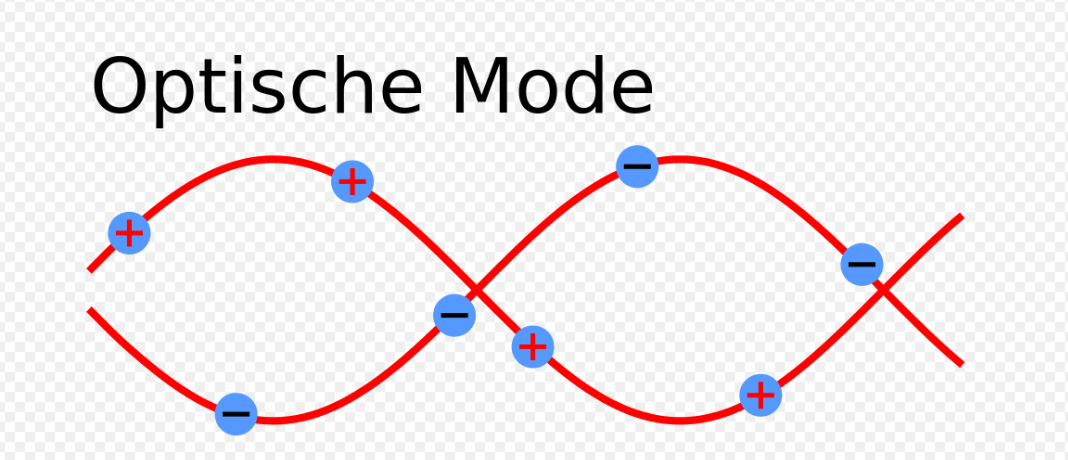
\includegraphics[width=0.8\linewidth]{resources/09-05-2012/opt.PNG}
            \caption{Darstellung von optischen Phononen}
          \end{figure}
\end{itemize}



\question{Vergleiche die Einstein- und Debye-Modelle der spez. Wärme. Welche Annahme ist im 
Einstein Modell zu einfach?}
\label{q:30}

\begin{figure}[H]  
    \centering
    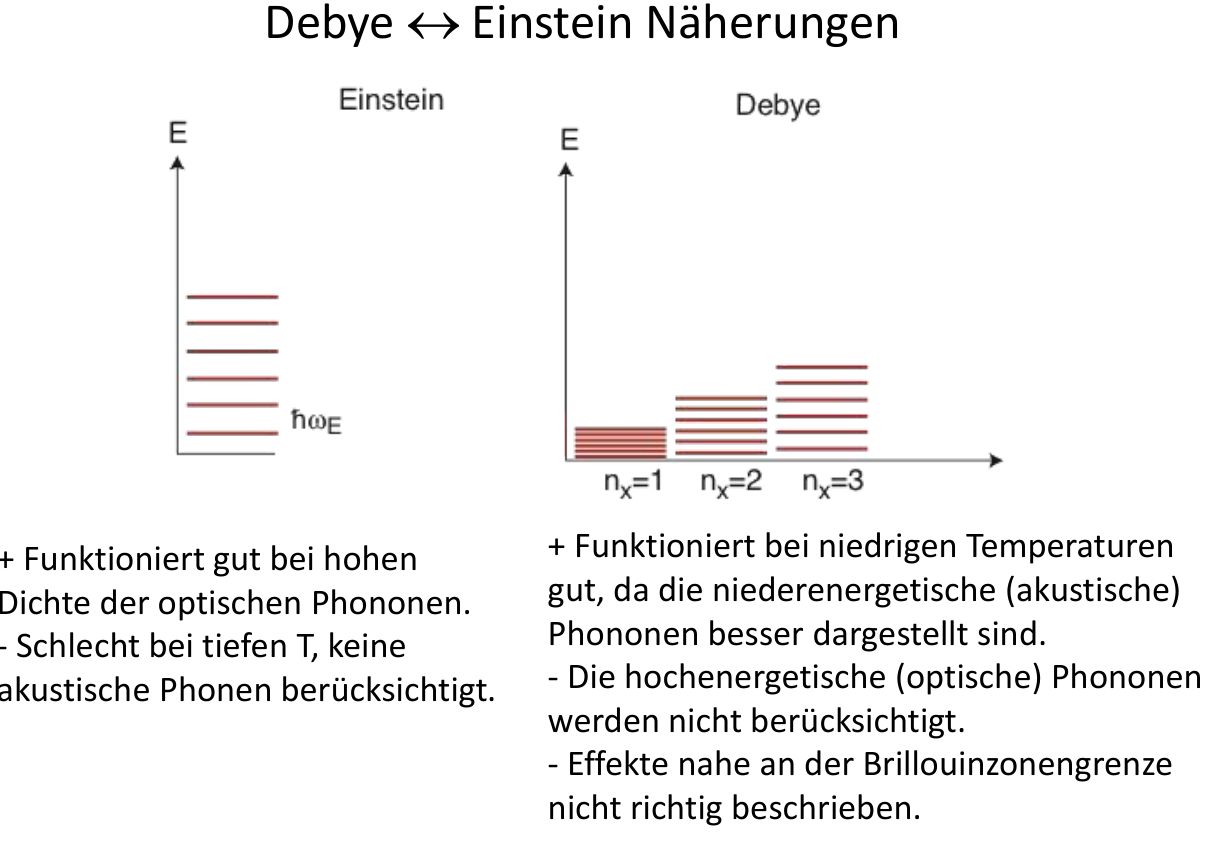
\includegraphics[width=.8\textwidth]{resources/09-05-2012/q30.png}
    \caption{Vergleich zwischen Einstein- und Debye-Modell.}
\end{figure}

Das Einsteinmodell nimmt an, dass alle Atome im Kristall mit der gleichen Frequenz schwingen, zudem werden keine akustischen Phononen berücksichtigt.

\newpage
\section{15. Juni 2015}

\question{Elektronenkonfiguration von $B_2$ ($Z=5$)}
\label{q:31}

$B_2$ = $1\sigma_g^2 ~ 1\sigma_u^{*2} ~ 2\sigma_g^2 ~ 2\sigma_u^{*2} ~ 1\pi_u^2$ \\

\begin{figure}[H]
    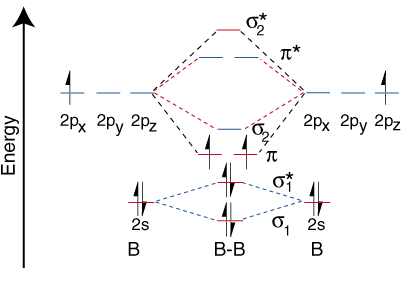
\includegraphics[width=0.8\linewidth]{resources/15-06-2015/b2.PNG}
    \caption{Elektronenkonfiguration von $B_2$}
\end{figure}

\question{Arten von Para-Diamagnetismus}
\label{q:32}

\question{Konzept von Bravais Wigner-Seitz Zelle}
\label{q:33}

Die Bravais Wigner-Seitz Zelle ist definiert als die Zelle im Raum, die jedem Gitterpunkt am nächsten 
liegt. Sie hat die folgenden Eigenschaften:
\begin{enumerate}
    \item Symmetrie: Die Zelle ist symmetrisch um den Gitterpunkt, von dem aus sie konstruiert wurde, sie weist alles Symmetrieoperationen, welche im gesamten Gitter vorkommen, auf. 
    \item Ein Gitterpunkt pro Zelle: Die Zelle enthält genau einen Gitterpunkt im Inneren der Zelle. Alle anderen Gitterpunkte des Gitters liegen auf den Seitenflächen der Zelle.
    \item Nächste Nachbarn: Die Zelle teilt den Raum so auf, dass jeder Gitterpunkt seinem nächstgelegenen Nachbarn am nächsten ist.
\end{enumerate}

Konstruktion:
\begin{figure}[H]
    \centering
    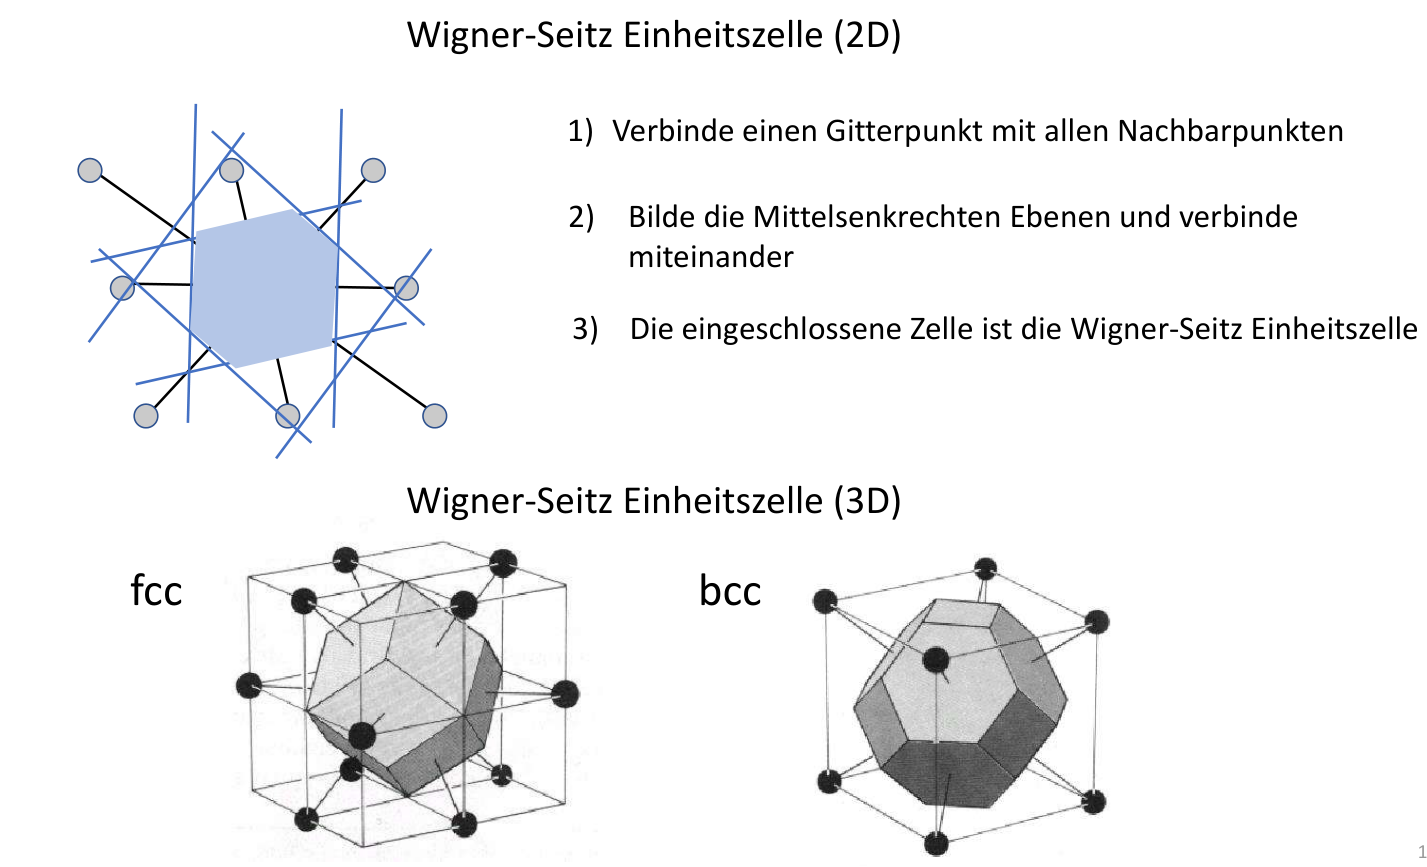
\includegraphics[width=0.8\linewidth]{resources/15-06-2015/q33.png}
    \caption{Konstruktion der Wigner-Seitz Zelle}
\end{figure}

\question{Sp sp2 sp3 Bindungen von mehratomigen Molekülen}
\label{q:34}

\question{Debye-Petit (oder so, irgendwas mit spezifischer Wärme von Elektronen)}
\label{q:35}

\question{Atom/Struktur Faktor}
\label{q:36}

\question{Zustandekommen von Energiebändern und Bandlöchern}
\label{q:37}

\question{Zusammenhang zwischen Gitterebene und Vektoren im reziproken Gitter}
\label{q:38}

Siehe \aqref{4}.

\question{Statische Abschirmung des Elektronengases}
\label{q:39}

\question{Einstein-Debye Unterschiede und falsche Annahmen}
\label{q:40}
\textbf{Einstein-Näherung} 
\begin{itemize}
    \item Annahme: alle Atome im Kristall schwingen mit der gleichen Frequenz $\omega$ = $\omega_E$, wobei $\omega_E$ die Frequenz der optischen Moden darstellt. 
    \item lässt sich nur auf optische Moden anwenden (nicht auf akkustische!)
    \item funktioniert gut bei hoher Dichte der optischen Phononen und liefert richtiges 
    Hochtermperaturlimit nach Dulong-Petit-Gesetz
    \item funktioniert schlecht bei tiefen Temperaturen und liefert ungenaues Limit für niedrige Temperaturen
    \item Falsche Annahme: akkustische Moden werden nicht berücksichtigt und alle harmonischen Oszillatoren im Festkörper würden mit einheitlicher Frequenz schwingen.
\end{itemize}

\textbf{Debye-Näherung} 
\begin{itemize}
    \item Annahme: 
        \begin{itemize}
            \item Vielzahl möglicher Frequenzen und Ausbreitungsgeschwindigkeit $v_i$ von Wellen/Phononen. 
            \item Lineare Dispersion $\omega_i=v_ik$ 
        \end{itemize}
    \item berücksichtigt nur akkustische Moden
    \item funktioniert gut bei niedrigen Temperaturen, da niederenergetische (akkustische) Phononen besser dargestellt sind 
    \item liefert korrektes Limit für hohe und tiefe Temperaturen
    \item Falsche Annahme: optische Phononen werden nicht berücksichtigt und Effekte nahe der Brillouinzonengrenze werden nicht richtig beschrieben
\end{itemize}

\begin{figure}[H]
 \centering
 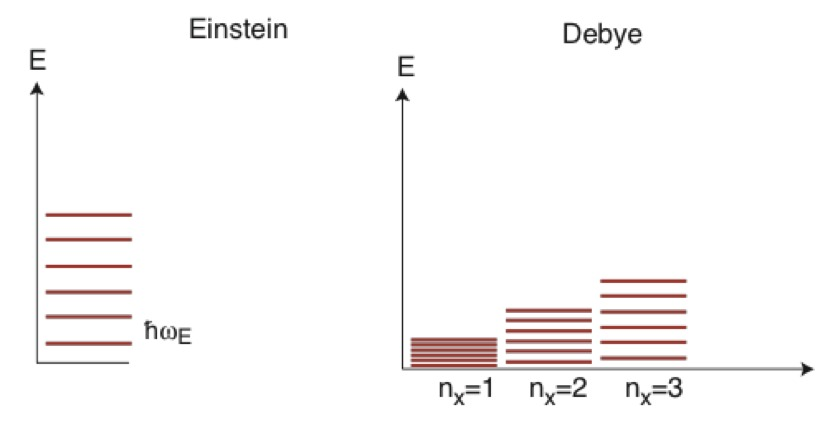
\includegraphics[width=0.6\textwidth]{resources/15-06-2015/Einstein_Debye.jpeg}
 \caption{Einstein- vs. Debye-Modell}
 %\label{}
\end{figure}
\newpage
\section{16. März 2012}

\question{Diskutieren der unterschiedlichen Überlegungen in der Valenzbindugsnäherung (VB) und in der Molekularorbitalnäherung (MO) zur Beschreibung der Molekülbindung in einem 2-atomigen Molekül}
\label{q:41}
\textbf{VB-Näherung}
\begin{itemize}
   
    \item erklärt Paarung von Elektronen durch Überlappung von Orbitale und Pi- und Sigma-Bindungen
    \item erklärt Hybridorbitale, aber liefert KEINE Details über Molekülorbitale
    \item im Grundzustand können zwei Elektronen mit $\uparrow \downarrow$ Spins untergebracht werden
    \item zwei lokalisierte Elektronen um Kerne A und B
    \item beide Elektronen werden betrachtet, sodass für beide Wahrscheinlichkeitsamplituden $\Psi_1$ und $\Psi_2$ ein Produktansatz der Atomorbitale notwendig ist 
    \item Besetzung des Molekülorbitals wird mit Linearkombination von $\Psi_1$ und $\Psi_2$ durch Pauli-Prinzip erzwungen
\end{itemize}


\noindent
\textbf{MO-Näherung}
\begin{itemize}
    \item basiert auf bindenden und antibindenden Molekülorbitalen
    \item erklärt nicht die Hybridisierung des Orbitale
    \item ein Elektron betrachtet, dass sich in $\Phi_A$ als auch in $\Phi_B$ aufhalten kann, sodass für dieses Molekülorbital-Ansatz notwendig ist (wobei $\Phi_A$ und $\Phi_B$ atomare Wellenfunktionen)
    \item für Besetzung des Molekülorbitals mit zwei Elektronen wird Produktansatz verwendet
\end{itemize}
\question{Skizzieren der bindenden und antibindenden Wellenfunktionen in einem homonuklearen 2-atomigen Molekül}
\label{q:42}
\begin{figure}[H]
    \centering
   \begin{minipage}[b]{.4\linewidth} % [b] => Ausrichtung an \caption
      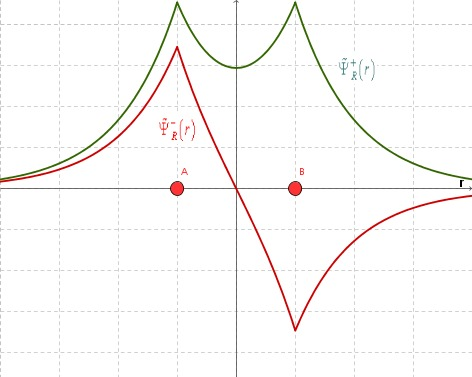
\includegraphics[width=\linewidth]{resources/16-03-2012/sym_und_antisymm_Wellenfunktion.jpeg}
      \caption{\textbf{Wellenfunktionen} symmetrische (bindend, grün) und antisymmetrische (antibindende, rot) Wellenfunktion}
   \end{minipage}
   \hspace{.1\linewidth}% Abstand zwischen Bilder
   \begin{minipage}[b]{.4\linewidth} % [b] => Ausrichtung an \caption
      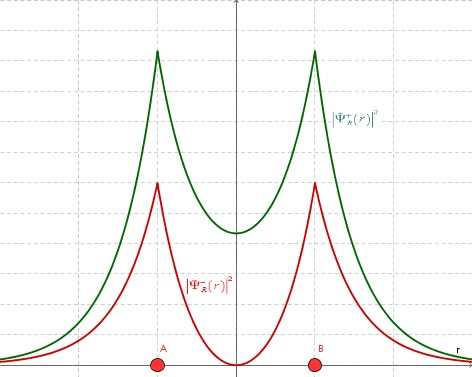
\includegraphics[width=\linewidth]{resources/16-03-2012/Wahrscheinlichkeitsdichten.jpeg}
      \caption{Wahrscheinlichkeitsdichten der symmetrischen (bindend, grün) und antisymmetrischen (antibindende, rot) Wellenfunktion}
   \end{minipage}
\end{figure}
\question{Diskutieren des Schwigungs-Rotations Spektrums eines 2-atomigen Moleküls}
\label{q:43}

\question{Diskutiere die chemische Bindung im Li2 Molekül}
\label{q:44}

\question{Was versteht man unter dem Franck-Condon Prinzip? Diskutiere die Intensität von Schwingungsbänden in einem Molekülspektrum bei einem elektronischen Übergang an Hand des Franck-Condon Prinzips.}
\label{q:45}

\question{Wodurch unterscheidet sich ein fcc Gitter von einem hcp?}
\label{q:46}

fcc- face centered cubic, hcp - hexagonal close packed

\begin{enumerate}
    \item Anordnung der Atome: Im fcc-Gitter sind die Atome auf den Eckpunkten eines Würfels sowie in den Zentren der sechs Flächen platziert. Im hcp-Gitter sind die Atome hexagonal angeordnet.
    \item Einheitszelle: Im fcc-Gitter ist die Einheitszelle ein Würfel, jeder Eckpunkt enthält ein Atom. Im hcp-Gitter ein hexagonales Prisma, jede Basiseben enthält ein Atom.
    \item Schichstruktur: Im fcc-Gitter gibt es keine klaren Schichten, da die Atome gleichmäßig im Raum verteilt sind. Im hcp-Gitter sind die Schichten klar definiert.
    \item Komprimierung: Im fcc-Gitter beträgt a:c : $\sqrt{2}:1$. Im hcp-Gitter beträgt a:c : $\sqrt{3}:2$.
\end{enumerate}

\question{Erläutere den Atomfaktor und den Strukturfaktor bei der Röntgenbeugung.}
\label{q:47}

\question{Skizziere die 1. Brillouin Zone eines ebenen Parallelogrammgitters.}
\label{q:48}

\question{Wodurch unterscheidet sich die Dispersionsrelation der Phononen eines primitiven kubischen Gitters von jener eines CsCl-Gitters.}
\label{q:49}

\question{Vergleiche die Einstein- und Debye-Modelle der spez. Wärme. Welche Annahme ist im Einstein Modell zu einfach?}
\label{q:50}

\newpage
\section{24. März 2015}

\question{Franck Condon Prinzip \& Intensität der Übergänge}
\label{q:51}

\question{Diskutiere die Elektronenkonfiguration von N2.}
\label{q:52}

N$_2$: $1\sigma_g^2 ~ 1\sigma_u^{*2} ~ 2\sigma_g^2 ~ 2\sigma_u^{*2} ~ 1\pi_u^4 ~ 3\sigma_g^2$ \\
14 Elektronen werden auf die $\pi$- und $\sigma$-Bindungen aufgeteilt. Achtung: Die Reihenfolge der $1\pi$- und der $3\sigma$-Orbitale kann variieren. Die unterschiedliche Reihenfolge dieser Orbitale kommt durch eine Mischung der s- und p-Atomorbitale zustande: Eine solche kann vorkommen, wenn der energetische Unterschied zwischen dem 2s- und dem 2p-Orbital der Atome klein genug ist (N$_2$ bildet genau die Grenze, bis zu der die Bildung dieser Mischung möglich ist). Dadurch wird zwar das $2\sigma_g$-Orbital stärker bindend, das $3\sigma_g$ wird jedoch schwächer bindend. Dadurch ist das $1\pi_u$-Orbital energetisch günstiger als das $3\sigma_g$ (\autoref{fig:q52}). Ist der (energetische) Abstand zwischen den s- und p-Atomorbitalen groß genug, so kann die Mischung der Orbitale vernachlässigt werden.

\begin{figure}[H]  
    \centering
    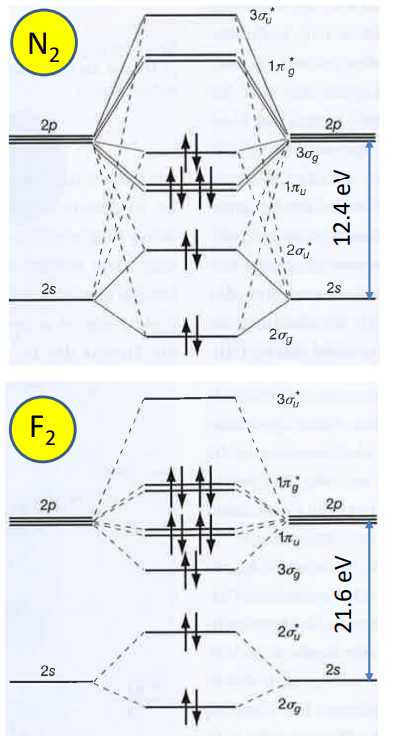
\includegraphics[width=.4\textwidth]{resources/24-03-2015/N2-F2.png}
    \caption{Elektronische Struktur von N$_2$ und F$_2$.}
    \label{fig:q52}
\end{figure}


\question{Diskutiere die Van der Waals Wechselwirkung und das Lennard-Jones Potential.}
\label{q:53}

Befindet sich ein neutrales Atom in einem elektrischen Feld $\vb{E}$, so induziert das Feld ein Dipolmoment $\vb{p_{ind}}$. Umgekehrt kann durch ein bestehendes Dipolmoment $\vb{p_A}$ aber auch ein elektrisches Feld entstehen - aus der Multipolentwicklung des elektrischen Feldes einer Ladungsverteilung ergibt sich für den Dipolanteil:
\begin{equation*}
    \vb{E}(\vb{p_A}) = \frac{1}{4\pi\varepsilon_0 R^3} (3 p_A \vb{\hat{R}} \cos{\theta_A} - \vb{p_A})
\end{equation*}
Ein neutrales Atom mit kugelsymmetrischer Elektronenhülle weist über die Zeit gemittelt aufgrund der Bewegung der Elektronen kein Dipolmoment auf - trotzdem hat ein solches Atom immer ein momentanes Dipolmoment. Dadurch entsteht ein elektrisches Feld, welches in einem anderen neutralen Atom ein Dipolmoment induzieren kann. Diese Wechselwirkung neutraler Atome ist die van-der-Waals-Wechselwirkung. Sie ist relativ schwach im Vergleich zu einer Ionenbindung und vor allem kurzreichweitig. Für das van-der-Waals-Potential gilt:
\begin{equation*}
    E_{pot}(R) = -\frac{C}{R^6}
\end{equation*}
Um das Potential noch besser zu beschreiben wird das empirisch ermittelte Lennard-Jones-Potential verwendet, das zusätzlich zum anziehenden Term des van-der-Waals-Potenzials noch einen abstoßenden Term berücksichtigt:
\begin{equation*}
    E_{pot}(R) = \frac{a}{R^{12}} - \frac{b}{R^6}
\end{equation*}
Dabei sind $a$ und $b$ Anpassungsparameter, die so gewählt werden, dass das Potenzial dem experimentell bestimmten Potenzial in möglichst guter Näherung entspricht. Durch die Kombination von anziehendem und abstoßendem Term entsteht ein Minimum des Potenzials beim Bindungsabstand mit $E_B = E_{pot}(R_e) = \frac{b^2}{2a}$.


\question{Konzept des Bravaisgitters und der Wigner-Seitz Zelle.}
\label{q:54}

Ein Bravaisgitter ist ein rein mathematisches Gitter, welches die Periodizität eines Kristallgitters beschreiben soll. An die einzelnen Gitterpunkte des periodischen Bravaisgitters können im Prinzip beliebig komplizierte Kombinationen von Atomen oder Molekülen gesetzt werden, die dann als Basis bezeichnet werden. Das Bravaisgitter beschreibt also nur die Periodizität, die Basis beschreibt die konkrete Struktur des Kristalls. Wichtig: Die Anordnung und Orientierung der Punkte im Bravaisgitter müssen identisch sein, egal von welchem Punkt man es betrachtet.

In einem solchen Gitter lassen sich unterschiedliche Arten von Einheitszellen definieren. Die Wigner-Seitz-Zelle lässt sich konstruieren, indem man:
\begin{itemize}
    \item ein Atom mit allen seinen Nachbarn verbindet
    \item Die Mittelsenkrechte auf alle Verbindungslinien konstruiert (in 3D entspricht das einer Ebene)
    \item Die von diesen Flächen eingeschlossene Fläche entspricht dann der Wigner-Seitz-Einheitszelle
\end{itemize}
Anmerkung: Konstruiert man die Wigner-Seitz-Einheitszelle im reziproken Gitter, so entspricht diese der 1. Brillouin-Zone.

\question{Diskutiere den Unterschied zwischen der akustischen und optischen Phononendispersionsrelation bzw. longitudinaler/transversaler, akustischer und optischer Phononen.}
\label{q:55}

Betrachtet man eine eindimensionale Kette aus zwei abwechselnd aufeinander folgenden Atomen $M_1$ und $M_2$, welche durch eine Hook'sche Feder verbunden sind, und löst die zugehörige Bewegungsgleichung, so ergibt sich daraus eine quadratische Gleichung für die Frequenz $\omega$. Die beiden Lösungen dieser Gleichung sind der optische und der akustische Ast, wobei der optische Ast nur dann auftritt, wenn die Kette tatsächlich aus einer zweiatomigen Basis besteht. Bei einer einatomigen Basis gibt es nur den akustischen Ast. Der optische Ast weist außerdem eine höhere Frequenz auf. Durch die unterschiedliche räumliche Orientierung der Schwingung lassen sich der akustische und der optische Ast weiters in transversale und longitudinale Äste einteilen. Bei $s$ Atomen pro Einheitszelle ergeben sich immer $3$ akustische Freiheitsgrade und $3s-3$ optische Freiheitsgrade (also insgesamt $3s$ Schwigungsäste).
% eventuell noch ausbaufähig

\question{Diskutiere das statische Verhalten des freien Elektronengases.}
\label{q:56}

Eine der Annahmen des klassischen Drude-Modells zur Beschreibung der Elektronen als freies Elektronengas schließt Kollisionen zwischen Elektronen aus und beschränkt sich somit nur auf Stöße zwischen Elektronen und Atomrümpfen. Letztere werden dabei als statisch betrachtet. Im Modell werden zusammengefasst die folgenden Annahmen getroffen:

\begin{enumerate}
    \item ideales Elektronengas: Keine WW zwischen den Elektronen
    \item Elektronen kollidieren nur mit Atomrümpfen, nicht untereinander
    \item Die Geschwindigkeit der Elektronen nach einem Stoß entspricht der Temperatur und sind damit vom herrschenden thermodynamischen Gleichgewicht abhängig
    \item Die mittlere freie Weglänge liegt in der Größenordnung der Atomabstände
\end{enumerate}

\question{Diskutiere die Einstein- und Debye-Näherung der Wärmekapazität.}
\label{q:57}

\question{Diskutiere den Beitrag der Elektronen zur Wärmekapazität.}
\label{q:58}

\question{Was besagt das Bloch Theorem bzw. die Bloch Funktion?}
\label{q:59}

\question{Welche Arten von Dia- und Paramagnetismus kennen Sie?}
\label{q:60}

\newpage
\section{28. November 2018}
%! Hier gibts schon ein bisschen was hier: https://docs.google.com/document/d/1VvuRhqSy6umcpChijdMtuYw5qB0H7iJZGPXQbSMj6zA/edit
\question{Skizzieren Sie die wesentlichen Elemente der Born-Oppenheimer Näherung.}
\label{q:61}

Da die Atomkerne eine wesentlich größere Masse als die Elektronen haben und sich dadurch viel langsamer bewegen, ist es mit der Born-Oppenheimer
Näherung möglich die Positionen der Kerne zu fixieren. Somit lässt sich die molekulare Schrödingergleichung in eine für die Kerne und eine
für die Elektronen aufteilen.

\begin{itemize}
    \item Für die Elektronen stehen die Kerne still, wodurch ihre Lage als Parameter in das anziehende und abstoßende Potential eingeht.
        Somit hängen die elektronischen Eigenzustände und Energien nur von der Lage der Kerne ab und nicht von der Geschwindigkeit.\\
            Die Schrödingergleichung für die Elektronen lautet somit:
            
        \begin{align}
            \hat{H}_e * \Phi_h(\vec{r},\vec{R}) = E_h(\vec{R}) *  \Phi_h(\vec{r},\vec{R})
        \end{align}

        Dabei ist $\vec{r}$ die Position der Elektronen und $\vec{R}$ die der Kerne. Der Hamiton besteht aus $\hat{H}_e = \hat{T}_e + \hat{V}_{ee} + \hat{V}_{eN}$, 
        also der kinetischen Energie der Elektronen + der Abstoßung zwischen den Elektronen + der Anziehung zwischen Kernen und Elektronen.

        \begin{figure}[H]
            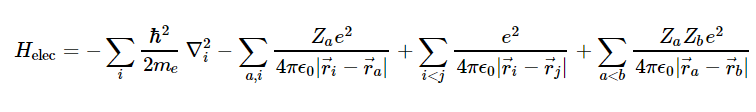
\includegraphics[width=0.8\linewidth]{resources/09-05-2012/born_op.PNG}
            \caption{Elektronischer Hamiton}
        \end{figure}

    \item Die Kernbewegeung ist von den Elektronen nahezu unbeeinflusst, jedoch bewegen sie sich im Potential der elektrischen Zustände. 
        Die Kern-Wellenfunktion $\eta_{hk}(\vec{R})$ hängt nur von der Kernkoordinate $\vec{R}$ ab.\\
        Die Schrödingergleichung lautet: 

        \begin{align}
            (\hat{T}_n + \hat{V}_{NN} + E_h(\vec{R})) * \eta_{hk}(\vec{R}) = E_{hk} * \eta_{hk}(\vec{R})
        \end{align}
\end{itemize}


\question{Diskutieren Sie die sp-, sp2-, sp3-Hybridisierung in mehratomigen Molekülen.}
\label{q:62}

Hybridisierung bedeutet eine Mischung aus s- und p- Orbitalen,
hervorgerufen durch die Verformung der Elektronenhülle auf Grund
der Wechselwirkung zwischen den an der Bindung beteiligten Atomen.
Dabei gibt es die sp-, die sp2- und die sp3-Hybridisierung:

\begin{itemize}
    \item Eine sp-Hybridisierung führt zu zwei entgegengerichteten Bindungen und damit
          zu einem linearen Molekül, wenn keine anderen Bindungen vorhanden sind. Hier hybridisieren das 2s und ein 2p Orbital zu zwei sp-Orbitalen.
         
          \begin{figure}[H]
            \begin{minipage}[b]{0.5\linewidth} 
               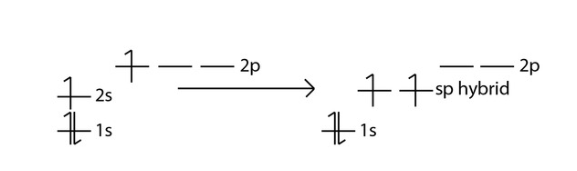
\includegraphics[width=0.8\linewidth]{resources/28-11-2018/sp11.PNG}
               \caption{sp-Hybridisierung, wobei die Energie sinkt}
            \end{minipage}
            \hspace{0.01\linewidth}
            \begin{minipage}[b]{0.5\linewidth} 
               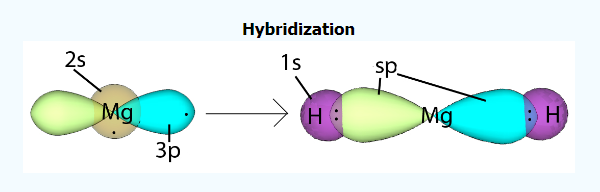
\includegraphics[width=0.8\linewidth]{resources/28-11-2018/sp12.PNG}
               \caption{sp-Hybridisierung am Beispiel von Magnesium }
            \end{minipage}
         \end{figure}

    \item Die sp2-Hybridisierung führt zu drei gerichteten Bindungen, die in einer
          Ebene liegen. Hier bilden sich aus den 2s und zwei 2p-Orbitalen, drei sp-Orbitale.

          \begin{figure}[H]
            \begin{minipage}[b]{0.5\linewidth} 
               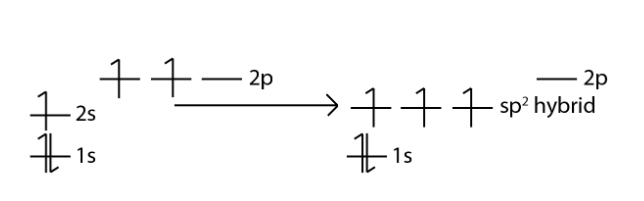
\includegraphics[width=0.8\linewidth]{resources/28-11-2018/sp21.PNG}
               \caption{sp2-Hybridisierung, wobei die Energie sinkt}
            \end{minipage}
            \hspace{0.01\linewidth}
            \begin{minipage}[b]{0.5\linewidth} 
               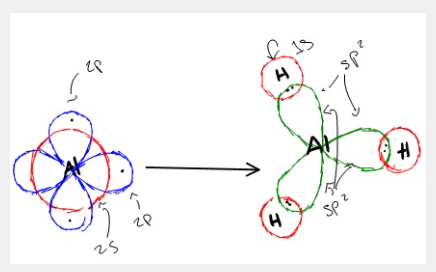
\includegraphics[width=0.8\linewidth]{resources/28-11-2018/sp22.PNG}
               \caption{sp2-Hybridisierung am Beispiel von Aluminiumhydroxid}
            \end{minipage}
         \end{figure}

    \item Für die sp3-Hybridisierung ergeben sich Atomorbitale mit Maxima, die in die vier Ecken eines Tetraeders zeigen.
          Hier bilden sich aus den 2s und drei 2p-Orbitalen, vier sp3-Orbitale.

          \begin{figure}[H]
            \begin{minipage}[b]{0.5\linewidth} 
               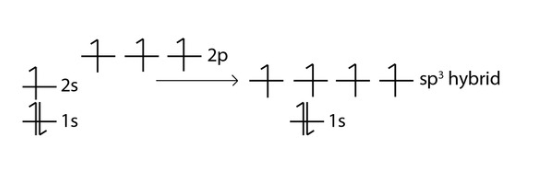
\includegraphics[width=0.8\linewidth]{resources/28-11-2018/sp31.PNG}
               \caption{sp3-Hybridisierung, wobei die Energie sinkt}
            \end{minipage}
            \hspace{0.01\linewidth}
            \begin{minipage}[b]{0.5\linewidth} 
               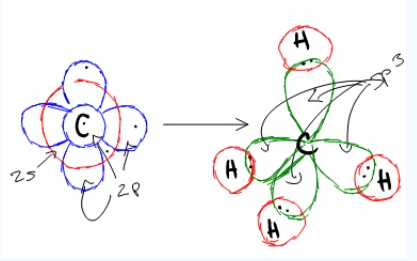
\includegraphics[width=0.8\linewidth]{resources/28-11-2018/sp32.PNG}
               \caption{sp3-Hybridisierung am Beispiel von Methan}
            \end{minipage}
         \end{figure}

\end{itemize}

\question{Diskutieren Sie die Laue'sche Beugungsbedingung anhand der Ewald-Konstruktion im Rahmen der Bragg'schen Interpretation.}
\label{q:63}

\question{Wodurch unterscheiden sich ein fcc-Gitter von einer hcp-Struktur?}
\label{q:64}

\question{Diskutieren Sie die Gitterenergie der Ionenkristalle.}
\label{q:65}

\question{Vergleichen Sie die Einstein- und Debye-Modelle der spezifischen Wärme. Welche Annahmen sind in beiden Modellen zu einfach?}
\label{q:66}

\question{Diskutieren Sie das Auftreten einer Energiebandlücke mit Hilfe des Modells der fast freien Elektronen.}
\label{q:67}

\question{Wodurch unterscheidet sich die Dispersionsrelation der Phononen eines primitiven kubischen Gitters von jenem eines CsCl-Gitters.}
\label{q:68}

\question{Erklären Sie die chemische Bindung von $O_2$ (O; $Z=8$).}
\label{q:69}

\newpage
\section{31. Oktober 2013}

\question{Bindungszustände / Elektronenkonfiguration in N2 diskutieren.}
\label{q:70}
Siehe \qref{52}.

\question{Skizzieren Sie die wesentlichen Elemente der Born-Oppenheimer Näherung.}
\label{q:71}

\question{Erklärung von Hybridisierung anhand sp, sp2 und sp3.}
\label{q:72}

\question{Lennard-Jones Potential und Van der Waals Bindung.}
\label{q:73}

\question{Diskutieren Sie die Laue'sche Beugungsbedingung.\
\label{q:74}
\qquad \qquad a) Anhand der Ewald-Konstruktion.\
\qquad \qquad b) Im Rahmen der Bragg'schen Interpretation.}

\question{Skizzieren Sie die 1. Brillouin-Zone eines ebenen hexagonalen Gitters.}
\label{q:75}

\question{Gitterenergie in einem Ionenkristall.}
\label{q:76}

\question{Röntgenbeugung mit der Drehkristallmethode.}
\label{q:77}

\question{Vergleichen Sie das Einstein- und Debye-Modell der spezifischen Wärme. Welche Annahme ist in BEIDEN Modellen zu einfach?}
\label{q:78}

\newpage
\section{Juli 2017}

\question{Zeichne das Potential eines homöopolaren Moleküls. Beschreiben Sie es qualitativ.}
\label{q:79}

\question{Was bewirkt die Austauschenergie beim H2 Molekül? Wann ist sie groß/klein? Wieso ist sie für die chemische Bindung wichtig?}
\label{q:80}

Siehe \aqref{1}.

\question{Was kann man aus dem Rotations-Schwingungsspektrum für molekulare Größen bestimmen?}
\label{q:81}

Siehe \aqref{2}.

\question{Diskutieren Sie elektrische Rotations-Schwingungsübergänge und die Entstehung von Schwingungsbanden.}
\label{q:82}

Siehe \aqref{3}.

\question{Wie kann experimentell die Dispersionsrelationskurve von Phononen ermittelt werden?}
\label{q:83}

\question{Diskutieren Sie die Wärmekapazität sowohl in der klassischen als auch in der quantenmechanischen Betrachtung.}
\label{q:84}

\question{Was für ein Zusammenhang besteht zwischen der Gitterebene und einem Vektor im reziproken Raum?}
\label{q:85}

Siehe \aqref{4}.

\question{Erklären Sie das Auftreten von Energiebandlücken mit Hilfe des Models der fast freien Elektronen.}
\label{q:86}

siehe \aqref{5}

\question{Beschreiben Sie das Bloch-Theorem eines Elektrons im harmonischen Potential.}
\label{q:87}

\question{Diskutieren Sie die Zustandsdichte in Schwingungsspektren von Festkörpern.}
\label{q:88}

\end{document}